\documentclass{article}

\usepackage{geometry}
\usepackage{amsmath}
\usepackage{graphicx}
\usepackage{listings}
\usepackage{hyperref}
\usepackage{multicol}
\usepackage{fancyhdr}
\pagestyle{fancy}
\hypersetup{ colorlinks=true, linkcolor=black, filecolor=magenta, urlcolor=cyan}
\geometry{ a4paper, total={170mm,257mm}, top=20mm, right=20mm, bottom=20mm, left=20mm}
\setlength{\parindent}{0pt}
\setlength{\parskip}{1em}
\renewcommand{\headrulewidth}{0pt}
\lhead{Competitive Programming - Arkavidia V}
\fancyfoot[CE,CO]{\thepage}

\begin{document}

\begin{center}
    \section*{J. Jelajah Indonesia} % ganti judul soal

    \begin{tabular}{ | c c | }
        \hline
        Batas Waktu  & 1s \\    % jangan lupa ganti time limit
        Batas Memori & 64MB \\  % jangan lupa ganti memory limit
        \hline
    \end{tabular}
\end{center}

\subsection*{Deskripsi}

Arvy dan teman-temannya menjelajahi Indonesia ke pulau Ganesha.
Di pulau ini, hanya ada $N$ kota yang dinomori dari $1$ sampai $N$.
Ada $N - 1$ jalan yang menyambungkan seluruh kota, yang mana semua jalan memiliki panjang yang sama.
Dijamin setiap kota dapat dicapai dari kota manapun.
Namun jarak antar kota ini cukup jauh, sehingga perjalanan bisa membosankan atau menyenangkan, tergantung pemandangan di sepanjang jalan.
Kita sebut dua kota yang disambungkan oleh sebuah jalan sebagai dua kota bertetangga.

Arvy ingin mengunjungi semua kota, sehingga ia akan mengambil rute dengan cara berikut:
\begin{enumerate}
    \item Arvy tiba di salah satu kota menggunakan pesawat.
    \item Setiap kali ia mengunjungi sebuah kota (sebut saja kota $X$), ia akan berada di sana selama sehari.
    \item Lalu, ia akan mencari satu kota terdekat yang belum pernah ia kunjungi dan bergerak ke sana, meskipun harus melewati kota yang pernah ia kunjungi.
    \item Ia akan melakukan hal ini terus hingga semua kota sudah dikunjungi.
\end{enumerate}
Tepat sesaat sesudah Arvy dan teman-temannya sudah mengunjungi semua kota, mereka akan pulang dari kota tersebut naik pesawat, jadi kota akhir perjalanan tidak harus sama dengan kota pertama yang dikunjungi.
Total keindahan sebuah rute mula-mula 0, dan bertambah sebesar $W$ jika ia melewati jalan dengan nilai keindahan $W$.

Kini ia harus bersiap-siap, karena perjalanan bisa sangat membosankan atau sangat indah.
Ia butuh bantuan untuk mencari tahu, berapakah total keindahan rute yang paling membosankan?

\subsection*{Format Masukan}
Baris pertama berisi bilangan positif $T$ ($T \leq 100$), menyatakan banyaknya kasus uji.
Untuk tiap kasus uji, baris pertama terdiri dari sebuah bilangan $N$ ($2 \leq N \leq 100.000$), menyatakan banyaknya kota pada pulau Ganesha.
$N-1$ baris berikutnya terdiri dari $U$ , $V$ ($1 \leq U, V \leq N$) dan $W$ ($-100.000 \leq W \leq 100.000$), menyatakan kota $U$ dan $V$ terhubung dengan jalan dengan nilai keindahan $W$.
Jalan dianggap membosankan jika nilai $W$ negatif, atau indah jika positif.

\subsection*{Format Keluaran}
Untuk tiap kasus uji, keluarkan sebuah bilangan dalam satu baris yang menyatakan total keindahan rute pada kasus terburuk.

\pagebreak

\begin{multicols}{2}
\subsection*{Contoh Masukan}
\begin{lstlisting}
2
7
3 4 9
1 2 3
2 7 2
3 6 1
2 3 8
3 5 5
5
1 2 -1
2 3 2
3 4 3
4 5 -5
\end{lstlisting}
\columnbreak
\subsection*{Contoh Keluaran}
\begin{lstlisting}
36
-6
\end{lstlisting}
\vfill
\null
\end{multicols}

\subsection*{Penjelasan}
Pada kasuss uji kedua, kota dapat digambarkan sebagai berikut:

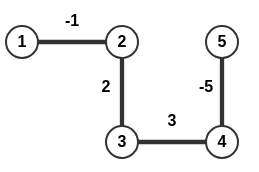
\includegraphics[width=150px]{sample-2}

Beberapa contoh rute:
\begin{itemize}
    \item \lstinline{1, 2, 3, 4, 5} dengan total keindahan $-1$.
    \item \lstinline{2, 1, 2, 3, 4, 5} dengan total keindahan $-2$.
    \item \lstinline{5, 4, 3, 2, 1} dengan total keindahan $-1$.
    \item \lstinline{4, 5, 4, 3, 2, 1} dengan total keindahan $-6$.
    \item dan lain-lain.
\end{itemize}

Dari semua rute yang valid, rute \lstinline{4, 5, 4, 3, 2, 1} merupakan rute dengan total keindahan paling membosankan (paling minimum).
Rute \lstinline{4, 5, 4, 3, 2, 1, 2} bukan merupakan rute yang valid karena seharusnya Arvy akan segera pulang sesaat sesudah mengunjungi semua kota (setelah sampai di kota $1$).

\pagebreak

\end{document}